\section{Approximation von $\pi$ mithilfe eines Monte Carlo Verfahren}
Wir wollen eine Approximation (Annäherung) der Kreiszahl $\pi$ mithilfe einer sogenannten \textit{Monte Carlo Methode} berechnen. Dazu betrachten wir die \textcolor{Blue!30}{Viertelkreisscheibe} in \cref{fig:Viertelkreisscheibe}, welche Teil des Einheitsquadrats ist. Die \textcolor{Red!30}{rote Fläche} ist derjenige Teil des Einheitsquadrats, welcher nicht zur \textcolor{Blue!30}{Viertelkreisscheibe} gehört.

\begin{myexercise}\label{myexercise:001}
	Wie gross ist die Fläche der Einheitskreisscheibe?
\end{myexercise}

\begin{figure}[H]
	\center
	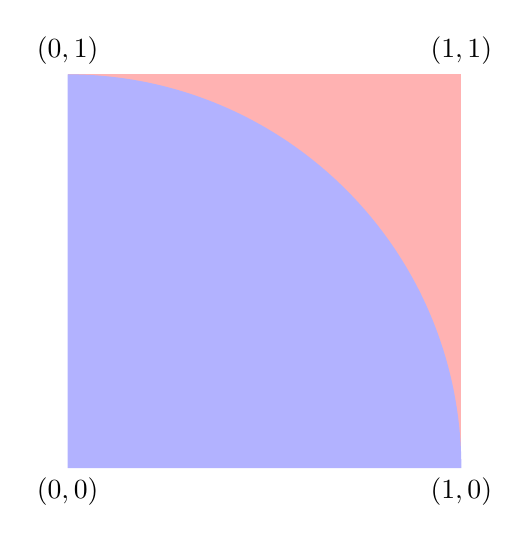
\begin{tikzpicture}[scale=5]
		% Draw the unit square
		% \draw[thick] (0,0) rectangle (1,1);
		\fill[Red!30](0,0) rectangle (1,1);

		% Draw the quarter-circle
		\fill[Blue!30] (0,0) -- (1,0) arc[start angle=0, end angle=90, radius=1cm] -- cycle; % Shaded quarter-circle
		% Labels for clarity
		\node at (1, 0) [below] {$(1,0)$};
		\node at (0, 1) [above] {$(0,1)$};
		\node at (0, 0) [below] {$(0,0)$};
		\node at (1, 1) [above] {$(1,1)$};
		% \node at (0.5, 0.5) [above right] {\tiny Quarter-Circle Area};
	\end{tikzpicture}
	\caption{Viertelkreisscheibe innerhalb des Einheitsquadrats}
	\label{fig:Viertelkreisscheibe}
\end{figure}

\begin{figure}[H]
	\center
	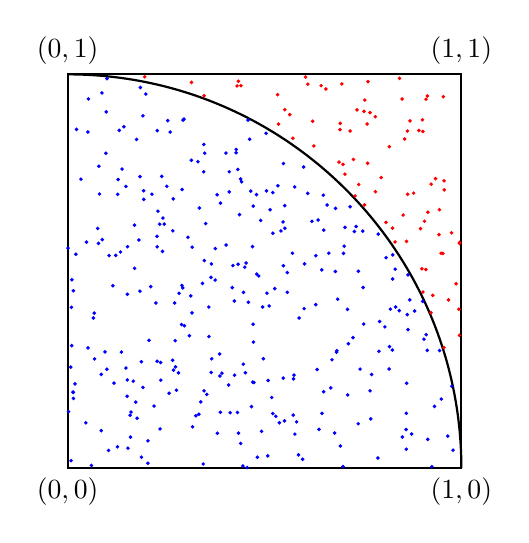
\begin{tikzpicture}[scale=5]
		% Draw the unit square
		\draw[thick] (0,0) rectangle (1,1);

		% Draw the quarter-circle
		% \draw (0,0) -- (1,0) arc[start angle=0, end angle=90, radius=1cm] -- cycle; % Shaded quarter-circle
		\draw[thick] (1,0) arc[start angle=0, end angle=90, radius=1cm];

		% Generate random points for Monte Carlo simulation
		\foreach \x in {1,...,400} {
				\pgfmathsetmacro{\px}{rnd}
				\pgfmathsetmacro{\py}{rnd}
				\ifdim \px pt<1pt
					\ifdim \py pt<1pt
						\pgfmathsetmacro{\dist}{sqrt(\px*\px + \py*\py)}
						\ifdim \dist pt<1pt
							\fill[blue] (\px, \py) circle(0.005cm); % Inside quarter-circle
						\else
							\fill[red] (\px, \py) circle(0.005cm); % Outside quarter-circle
						\fi
					\fi
				\fi
			}

		% Labels for clarity
		\node at (1, 0) [below] {$(1,0)$};
		\node at (0, 1) [above] {$(0,1)$};
		\node at (0, 0) [below] {$(0,0)$};
		\node at (1, 1) [above] {$(1,1)$};
		% \node at (0.5, 0.5) [above right] {\tiny Quarter-Circle Area};
	\end{tikzpicture}
	\caption{Generiere eine grosse Anzahl zufällig gewählter Punkte innerhalb des Einheitsquadrats. Punkte, welche innerhalb der Viertelkreisscheibe liegen, sind blau gefärbt. Punkte ausserhalb der Viertelkreisscheibe sind rot gefärbt.}
	\label{fig:monteCarlo}
\end{figure}



\clearpage
\section{Lösungen der Aufgaben}
\begin{myanswer}[myexercise:001]
	Der Flächeninhalt $A$ eines Kreises mit Radius $r$ ist gegeben durch $A = r^2\pi$. Da der Einheitskreis den Radius $r = 1$ hat, ist sein Flächeninhalt gegeben durch die Kreiszahl $\pi$.
\end{myanswer}
